\RequirePackage{luatex85}
\documentclass[border=1pt]{standalone}
\usepackage{tikz}
\usetikzlibrary{shapes.geometric, positioning, arrows}

%%%%%%%%%%%%%%%%%%%%%%%%%%%%%%%%%%%%%%%%%%%%%%%%%%%%%%%%%%%%%%%%%%%%%%%%%%%%%%%%
%%%%%%%%%%%%%%%%%%%%                 colours                %%%%%%%%%%%%%%%%%%%% 
%%%%%%%%%%%%%%%%%%%%%%%%%%%%%%%%%%%%%%%%%%%%%%%%%%%%%%%%%%%%%%%%%%%%%%%%%%%%%%%%

\definecolor{tugreen}{RGB}{128, 186, 38}
\definecolor{tucitron}{RGB}{249, 219, 0}



%%%%%%%%%%%%%%%%%%%%%%%%%%%%%%%%%%%%%%%%%%%%%%%%%%%%%%%%%%%%%%%%%%%%%%%%%%%%%%%%
%%%%%%%%%%%%%%%%%%%%                 Boxes                  %%%%%%%%%%%%%%%%%%%% 
%%%%%%%%%%%%%%%%%%%%%%%%%%%%%%%%%%%%%%%%%%%%%%%%%%%%%%%%%%%%%%%%%%%%%%%%%%%%%%%%
\tikzstyle{normalBox} = [shape=rectangle, draw=black, text=black, thick, 	
	align=center, fill=white]

\tikzstyle{roundBox} = [shape=circle, draw=black, text=black, thick, 	
	align=center, fill=white]

\tikzstyle{alternBox} = [shape=rectangle, text=white, thick, align=center, 
	fill=black, rounded corners]


%%%%%%%%%%%%%%%%%%%%%%%%%%%%%%%%%%%%%%%%%%%%%%%%%%%%%%%%%%%%%%%%%%%%%%%%%%%%%%%%
%%%%%%%%%%%%%%%%%%%%                 Arrows                 %%%%%%%%%%%%%%%%%%%% 
%%%%%%%%%%%%%%%%%%%%%%%%%%%%%%%%%%%%%%%%%%%%%%%%%%%%%%%%%%%%%%%%%%%%%%%%%%%%%%%%

\tikzstyle{normalArrow} = [thick,->,>=stealth, draw=black]

\usepackage[utf8]{inputenc}
\usepackage[T1]{fontenc}
\usepackage[sfdefault]{FiraSans}


\tikzstyle{NormalBox} = [normalBox, text width =2.5cm, minimum height=1cm]
\tikzstyle{AlternBox} = [alternBox, text width =2.5cm, minimum height=1cm]

\begin{document}
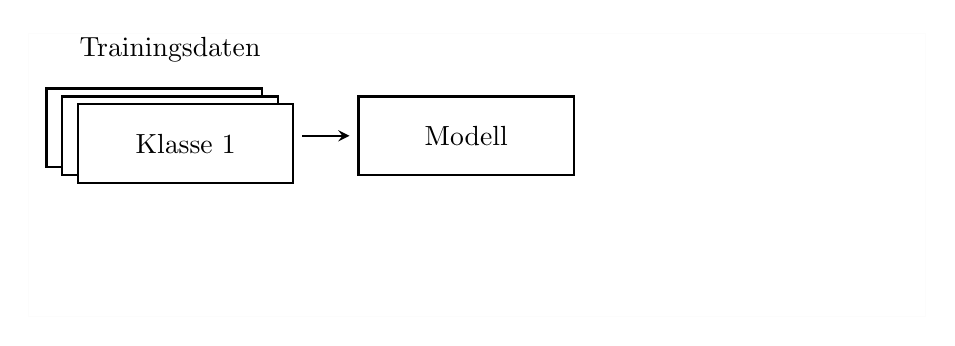
\begin{tikzpicture}[node distance=1cm]
   \draw[black!01] (-1.6,1.2) rectangle (9.8,-2.4);
  	\draw (0.2,1.) node[text=black] {Trainingsdaten};
	\node (Class1) at (0,0) [NormalBox] {Klasse 3};
	\node (Class2) at (Class1) [NormalBox, xshift=.2cm, yshift=-.1cm] {Klasse 2};
	\node (Class3) at (Class2) [NormalBox, xshift=.2cm, yshift=-.1cm] {Klasse 1};

	\node (Modell) [NormalBox, right= of Class2] {Modell};
	\draw [normalArrow,shorten <=.3cm,shorten >=.1cm] (Class2) -- (Modell);

%	\node (TDaten) [NormalBox, below= of Modell, yshift=0.3cm] {Testdaten};
%	\draw [normalArrow,shorten <=.1cm,shorten >=.1cm] (TDaten) -- (Modell);
%	
%	\node (Test1) [NormalBox, right= of Modell, xshift=.0cm, yshift=.1cm] {Klasse 3};
%	\node (Test2) [NormalBox, right= of Modell, xshift=.2cm, yshift=.0cm] {Klasse 2};
%	\node (Test3) [NormalBox, right= of Modell, xshift=.4cm, yshift=-.1cm] {Klasse 1};
%  	\draw (7.8,1.) node[text=black] {Klassifizierte Testdaten};
%	\draw [normalArrow,shorten <=.1cm,shorten >=.3cm] (Modell) -- (Test2);
\end{tikzpicture}
\end{document}
